% Title     :: SamzaSQL: Scalable Fast Data Management with Streaming SQL
% Author    :: Milinda Pathirage
% Email     :: mpathira@indiana.edu
% Website   :: http://milinda.pathirage.org
% Template  :: sthlm beamer theme by Benjamin Weiss (hendryolson@gmail.com, http://v42.com), 
%              which is HEAVILY based on the HSRM beamer theme created by Benjamin Weiss
%			   (benjamin.weiss@student.hs-rm.de), which can be found on GitHub
%			   <https://github.com/hsrmbeamertheme/hsrmbeamertheme>.



%-=-=-=-=-=-=-=-=-=-=-=-=-=-=-=-=-=-=-=-=-=-=-=-=
%
%        LOADING DOCUMENT
%
%-=-=-=-=-=-=-=-=-=-=-=-=-=-=-=-=-=-=-=-=-=-=-=-=

\documentclass[newPxFont]{beamer}
\usetheme{sthlm}
%\usecolortheme{sthlmv42}

%-=-=-=-=-=-=-=-=-=-=-=-=-=-=-=-=-=-=-=-=-=-=-=-=
%        LOADING PACKAGES
%-=-=-=-=-=-=-=-=-=-=-=-=-=-=-=-=-=-=-=-=-=-=-=-=
\usepackage[utf8]{inputenc}
\usepackage{hyperref}
\usepackage{minted}
\usepackage{xcolor}

\usepackage{chronology}

\renewcommand{\event}[3][e]{%
  \pgfmathsetlength\xstop{(#2-\theyearstart)*\unit}%
  \ifx #1e%
    \draw[fill=black,draw=none,opacity=0.5]%
      (\xstop, 0) circle (.2\unit)%
      node[opacity=1,rotate=45,right=.2\unit] {#3};%
  \else%
    \pgfmathsetlength\xstart{(#1-\theyearstart)*\unit}%
    \draw[fill=black,draw=none,opacity=0.5,rounded corners=.1\unit]%
      (\xstart,-.1\unit) rectangle%
      node[opacity=1,rotate=45,right=.2\unit] {#3} (\xstop,.1\unit);%
  \fi}%

%-=-=-=-=-=-=-=-=-=-=-=-=-=-=-=-=-=-=-=-=-=-=-=-=
%        BEAMER OPTIONS
%-=-=-=-=-=-=-=-=-=-=-=-=-=-=-=-=-=-=-=-=-=-=-=-=

%\setbeameroption{show notes}

%-=-=-=-=-=-=-=-=-=-=-=-=-=-=-=-=-=-=-=-=-=-=-=-=
%
%	PRESENTATION INFORMATION
%
%-=-=-=-=-=-=-=-=-=-=-=-=-=-=-=-=-=-=-=-=-=-=-=-=

\title{SamzaSQL}
\subtitle{Scalable Fast Data Management with \textit{Streaming SQL}}
%\date{\small{\jobname}}
%\date{\today}
\author{\textbf{Milinda Pathirage} (IU), Julian Hyde (Hortonworks), Yi Pan (LinkedIn), Beth Plale (IU)}
\institute{School of Informatics and Computing, Indiana University}

\hypersetup{
pdfauthor = {Milinda Pathirage: mpathira@indiana.edu},
pdfsubject = {},
pdfkeywords = {},
pdfmoddate= {D:\pdfdate},
pdfcreator = {}
}

\begin{document}
\setbeamertemplate{caption}{\raggedright\insertcaption\par}

%-=-=-=-=-=-=-=-=-=-=-=-=-=-=-=-=-=-=-=-=-=-=-=-=
%
%	TITLE PAGE
%
%-=-=-=-=-=-=-=-=-=-=-=-=-=-=-=-=-=-=-=-=-=-=-=-=

\maketitle

%\begin{frame}[plain]
%	\titlepage
%\end{frame}

%-=-=-=-=-=-=-=-=-=-=-=-=-=-=-=-=-=-=-=-=-=-=-=-=
%
%	TABLE OF CONTENTS: OVERVIEW
%
%-=-=-=-=-=-=-=-=-=-=-=-=-=-=-=-=-=-=-=-=-=-=-=-=

\section*{Introduction}

%-=-=-=-=-=-=-=-=-=-=-=-=-=-=-=-=-=-=-=-=-=-=-=-=
%	FRAME:
%-=-=-=-=-=-=-=-=-=-=-=-=-=-=-=-=-=-=-=-=-=-=-=-=

\begin{frame}[c]{Fast Data}

Data has to be process as it arrives, so that we can react to changing conditions fast. 

\vspace{1em}

\begin{exampleblock}{Big data isn't just big; it's also fast.}
Big data is often created by data that is generated at incredible speeds, such as click-stream data, financial ticker data, log aggregation, or sensor data. 
\end{exampleblock}
\vspace{-1.5em}
\begin{flushright}
\tiny\textit{John Hugg, \textbf{"Fast data: The next step after big data"}}
\end{flushright}

\end{frame}

%-=-=-=-=-=-=-=-=-=-=-=-=-=-=-=-=-=-=-=-=-=-=-=-=
%	FRAME:
%-=-=-=-=-=-=-=-=-=-=-=-=-=-=-=-=-=-=-=-=-=-=-=-=

\begin{frame}[c]{Lambda Architecture (LA)}
Technology agnostic data processing architecture that attempts to balance latency, accuracy, throughput and fault-tolerance by providing a unified serving layer on top of batch and stream processing sub-systems.   \\

\vspace{1em}

\begin{figure}
		\centering
		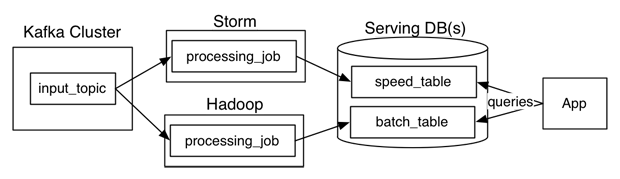
\includegraphics[width=0.75\linewidth]{lambda.png}
		\label{fig-lambda}
		\caption{\tiny\textit{From: \url{https://www.oreilly.com/ideas/questioning-the-lambda-architecture}}}
	\end{figure}

\end{frame}

%-=-=-=-=-=-=-=-=-=-=-=-=-=-=-=-=-=-=-=-=-=-=-=-=
%	FRAME:
%-=-=-=-=-=-=-=-=-=-=-=-=-=-=-=-=-=-=-=-=-=-=-=-=

\begin{frame}[c]{Kappa Architecture (KA)}
Simplification of \textit{Lambda Architecture} that uses append-only immutable log as the canonical data store and batch processing is replaced by stream replay. \\

\vspace{1em}

\begin{figure}
		\centering
		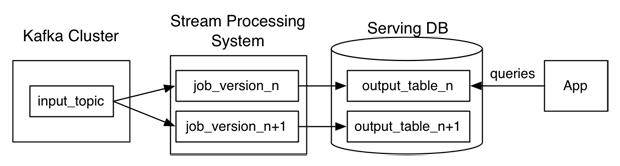
\includegraphics[width=0.75\linewidth]{kappa.png}
		\label{fig-kappa}
		\caption{\tiny\textit{From: \url{https://www.oreilly.com/ideas/questioning-the-lambda-architecture}}}
	\end{figure}

\end{frame}

%-=-=-=-=-=-=-=-=-=-=-=-=-=-=-=-=-=-=-=-=-=-=-=-=
%	FRAME:
%-=-=-=-=-=-=-=-=-=-=-=-=-=-=-=-=-=-=-=-=-=-=-=-=

%\begin{frame}[c]{sthlm Built on HSRM \& mTheme}
%\vspace{-1cm}
%\begin{center}\begin{chronology}[2]{2012}{2018}{0.85\textwidth}
%\event[\decimaldate{1}{1}{2013}]{\decimaldate{22}{9}{2013}}{hsrm theme}
%\event[\decimaldate{22}{9}{2013}]{\decimaldate{22}{8}{2014}}{sthlm based on hsrm}
%\event[\decimaldate{22}{8}{2014}]{\decimaldate{27}{4}{2015}}{branding sthlm for Stockholms stad}
%\event[\decimaldate{27}{4}{2015}]{\decimaldate{30}{8}{2015}}{\cRed{sthlm based on hsrm \& mTheme}}
%\end{chronology}
%\end{center}

%sthlm Theme is heavily based on the work of Benjamin Weiss \alert{HSRM} and Matthias Vogelgesang \alert{mTheme}.

%\end{frame}

%\section*{Overview}
%\begin{frame}{Overview}
% For longer presentations use hideallsubsections option
%\tableofcontents[hideallsubsections]
%\end{frame}


%-=-=-=-=-=-=-=-=-=-=-=-=-=-=-=-=-=-=-=-=-=-=-=-=
%
%	SECTION: Motivation
%
%-=-=-=-=-=-=-=-=-=-=-=-=-=-=-=-=-=-=-=-=-=-=-=-=

\section{Motivation}

%-=-=-=-=-=-=-=-=-=-=-=-=-=-=-=-=-=-=-=-=-=-=-=-=
%	FRAME: 
%-=-=-=-=-=-=-=-=-=-=-=-=-=-=-=-=-=-=-=-=-=-=-=-=

\begin{frame}{Programming APIs for LA and KA}

\href{https://github.com/twitter/summingbird}{\textbf{Summingbird}} is a well known abstraction for writing \textit{LA} style applications while \textit{KA} style applications were mainly written in \textbf{stateful stream processing APIs} provided by frameworks like \href{http://samza.apache.org}{Apache Samza}.

\begin{block}{Limitations}
\begin{itemize}
	\item Need to maintain two complex distributed systems
	\item Users need to understand complex programming abstractions 
	\item Long turnaround times
\end{itemize}
\end{block}

\end{frame}

%-=-=-=-=-=-=-=-=-=-=-=-=-=-=-=-=-=-=-=-=-=-=-=-=
%	FRAME: 
%-=-=-=-=-=-=-=-=-=-=-=-=-=-=-=-=-=-=-=-=-=-=-=-=

\begin{frame}[fragile]{Summingbird}
\begin{exampleblock}{Word Count}
\begin{minted}[
framesep=2mm,
baselinestretch=1.2,
fontsize=\footnotesize,
]{scala}
def wordCount[P <: Platform[P]]
    (source: Producer[P, String], store: P#Store[String, Long]) =
      source.flatMap { sentence =>
        toWords(sentence).map(_ -> 1L)
      }.sumByKey(store)
\end{minted}
\end{exampleblock}
\vspace{-1.5em}
\begin{flushright}
\tiny\textit{More examples at \url{https://github.com/twitter/summingbird}}
\end{flushright}
\end{frame}

%-=-=-=-=-=-=-=-=-=-=-=-=-=-=-=-=-=-=-=-=-=-=-=-=
%	FRAME: 
%-=-=-=-=-=-=-=-=-=-=-=-=-=-=-=-=-=-=-=-=-=-=-=-=

\begin{frame}[fragile]{Samza API}
\begin{exampleblock}{Window Aggregation}
\begin{minted}[
framesep=0mm,
%baselinestretch=1.2,
fontsize=\tiny,
]{java}
public class WikipediaStatsStreamTask implements StreamTask, InitableTask, WindowableTask {
  ...
  private KeyValueStore<String, Integer> store;
  public void init(Config config, TaskContext context) {
    this.store = (KeyValueStore<String, Integer>) context.getStore("wikipedia-stats");
  }
  @Override
  public void process(IncomingMessageEnvelope envelope, MessageCollector collector, 
                      TaskCoordinator coordinator) {
    Map<String, Object> edit = (Map<String, Object>) envelope.getMessage();
    ...
  }
  @Override
  public void window(MessageCollector collector, TaskCoordinator coordinator) {
    ...
    collector.send(new OutgoingMessageEnvelope(new SystemStream("kafka", "wikipedia-stats"), counts));
    ...
  }
\end{minted}
\end{exampleblock}

\end{frame}


%-=-=-=-=-=-=-=-=-=-=-=-=-=-=-=-=-=-=-=-=-=-=-=-=
%	FRAME:
%-=-=-=-=-=-=-=-=-=-=-=-=-=-=-=-=-=-=-=-=-=-=-=-=

\begin{frame}{SQL for Big Data}

There are sevaral well known SQL-on-Hadoop solutions and most organisations that use Hadoop use one or more SQL-on-Hadoop solutions.

\begin{itemize}
	\item Apache Hive
	\item Presto
	\item Apache Drill
	\item Apache Impala
	\item Apache Kylin
	\item Apache Tajo
	\item Apache Pheonix
\end{itemize}

\end{frame}


%-=-=-=-=-=-=-=-=-=-=-=-=-=-=-=-=-=-=-=-=-=-=-=-=
%	FRAME: 
%-=-=-=-=-=-=-=-=-=-=-=-=-=-=-=-=-=-=-=-=-=-=-=-=

\begin{frame}{Motivating Research Question}
\Large{Can the same low barrier and the clear semantics of SQL be extended to queries that execute simultaneously over data \texttt{\textbf{streams}} (in movement) and \texttt{\textbf{tables}} (at rest)?} \\

\Large{Can this be done with minimal and well-founded extensions to SQL?}
\end{frame}
%-=-=-=-=-=-=-=-=-=-=-=-=-=-=-=-=-=-=-=-=-=-=-=-=
%
%	SECTION: UPDATESS
%
%-=-=-=-=-=-=-=-=-=-=-=-=-=-=-=-=-=-=-=-=-=-=-=-=

\section{SamzaSQL}

%-=-=-=-=-=-=-=-=-=-=-=-=-=-=-=-=-=-=-=-=-=-=-=-=
%	FRAME:
%-=-=-=-=-=-=-=-=-=-=-=-=-=-=-=-=-=-=-=-=-=-=-=-=

\begin{frame}[c]{Streaming SQL - Data Model}

\begin{itemize}
	\item \textbf{Stream:} A stream S is a possibly indefinite par- titioned sequence of temporally-defined elements where an element is a tuple belonging to the schema of S.
	\item \textbf{Partition:} A partition is a time-ordered, immutable sequence of elements existing within a single stream.
	\item \textbf{Relation:} Analogous to a relation/table in relational databases, a relation R is a bag of tuples belonging to the schema of R. 
\end{itemize}

\end{frame}


%-=-=-=-=-=-=-=-=-=-=-=-=-=-=-=-=-=-=-=-=-=-=-=-=
%	FRAME:
%-=-=-=-=-=-=-=-=-=-=-=-=-=-=-=-=-=-=-=-=-=-=-=-=

\begin{frame}[fragile]{Streaming SQL - Continuous Queries}

\begin{alertblock}{SamzaSQL}
 \begin{minted}[
 framesep=2mm,
 baselinestretch=1.2,
 fontsize=\footnotesize,
 escapeinside=||]{sql}
 SELECT |\colorbox{yellow}{STREAM}| rowtime, productId, units FROM Orders 
   WHERE units > 25
 \end{minted}
\end{alertblock}

\begin{exampleblock}{CQL}
 \begin{minted}[
 framesep=2mm,
 baselinestretch=1.2,
 fontsize=\scriptsize]{sql}
 SELECT ISTREAM rowtime, productId, units FROM Orders 
   WHERE units > 25;
 \end{minted}
\end{exampleblock}
\end{frame}

%-=-=-=-=-=-=-=-=-=-=-=-=-=-=-=-=-=-=-=-=-=-=-=-=
%	FRAME:
%-=-=-=-=-=-=-=-=-=-=-=-=-=-=-=-=-=-=-=-=-=-=-=-=

\begin{frame}[fragile]{Streaming SQL - Window Aggregations}

\begin{alertblock}{SamzaSQL}
 \begin{minted}[
 framesep=2mm,
 baselinestretch=1.2,
 fontsize=\scriptsize,
 escapeinside=||]{sql}
 SELECT STREAM |\colorbox{yellow}{TUMBLE\_END}|(rowtime, INTERVAL '1' HOUR) AS rowtime,
   productId,
   COUNT(*) AS c,
   SUM(units) AS units
 FROM Orders
 GROUP BY |\colorbox{yellow}{TUMBLE}|(rowtime, INTERVAL '1' HOUR), productId
 \end{minted}
\end{alertblock}

\begin{exampleblock}{CQL}
 \begin{minted}[
 framesep=2mm,
 baselinestretch=1.2,
 fontsize=\scriptsize]{sql}
 SELECT ISTREAM ... AS rowtime, productId, COUNT(*) AS c, 
   SUM(units) AS units
 FROM Orders[Range '1' HOUR, Slide '1' HOUR]
 GROUP BY  productId;
 \end{minted}
\end{exampleblock}

\end{frame}

%-=-=-=-=-=-=-=-=-=-=-=-=-=-=-=-=-=-=-=-=-=-=-=-=
%	FRAME:
%-=-=-=-=-=-=-=-=-=-=-=-=-=-=-=-=-=-=-=-=-=-=-=-=

\begin{frame}[fragile]{Streaming SQL - Sliding Windows}

\begin{alertblock}{SamzaSQL}
 \begin{minted}[
 framesep=2mm,
 baselinestretch=1.2,
 fontsize=\scriptsize,
 escapeinside=||]{sql}
 SELECT STREAM rowtime, productId, units,
   SUM(units) |\colorbox{yellow}{OVER}| (ORDER BY rowtime PARTITION BY productId RANGE
     INTERVAL '1' HOUR PRECEDING) unitsLastHour 
 FROM Orders;
 \end{minted}
\end{alertblock}

\begin{exampleblock}{CQL}
 \begin{minted}[
 framesep=2mm,
 baselinestretch=1.2,
 fontsize=\scriptsize]{sql}
 SELECT ISTREAM rowtime, productId, units, 
   SUM(units) AS unitsLastHour
 FROM Orders[Range '1' HOUR]
 GROUP BY  productId;
 \end{minted}
\end{exampleblock}

\end{frame}

%-=-=-=-=-=-=-=-=-=-=-=-=-=-=-=-=-=-=-=-=-=-=-=-=
%	FRAME:
%-=-=-=-=-=-=-=-=-=-=-=-=-=-=-=-=-=-=-=-=-=-=-=-=

\begin{frame}[fragile]{Streaming SQL - Window Joins}

\begin{alertblock}{SamzaSQL}
 \begin{minted}[
 framesep=2mm,
 baselinestretch=1.2,
 fontsize=\scriptsize,
 escapeinside=||]{sql}
 SELECT STREAM
   GREATEST(PacketsR1.rowtime, PacketsR2.rowtime) AS rowtime,
   PacketsR1.sourcetime,
   PacketsR1.packetId,
   PacketsR2.rowtime - PacketsR1.rowtime AS timeToTravel
 FROM PacketsR1 JOIN PacketsR2 ON
   PacketsR1.rowtime BETWEEN
   PacketsR2.rowtime - INTERVAL '2' SECOND
   AND PacketsR2.rowtime + INTERVAL '2' SECOND
   AND PacketsR1.packetId = PacketsR2.packetId
 \end{minted}
\end{alertblock}

\end{frame}

%-=-=-=-=-=-=-=-=-=-=-=-=-=-=-=-=-=-=-=-=-=-=-=-=
%	FRAME:
%-=-=-=-=-=-=-=-=-=-=-=-=-=-=-=-=-=-=-=-=-=-=-=-=

\begin{frame}[c]{SamzaSQL - Architecture}
\begin{figure}
		\centering
		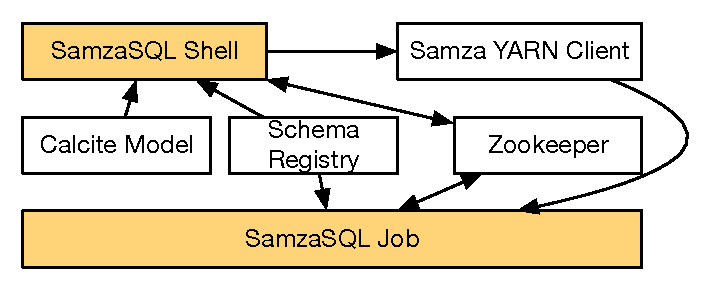
\includegraphics[width=0.9\linewidth]{samzasql-arch.pdf}
	\end{figure}
\end{frame}

%-=-=-=-=-=-=-=-=-=-=-=-=-=-=-=-=-=-=-=-=-=-=-=-=
%	FRAME:
%-=-=-=-=-=-=-=-=-=-=-=-=-=-=-=-=-=-=-=-=-=-=-=-=

\begin{frame}[c]{SamzaSQL - Query Planner}
\begin{figure}
		\centering
		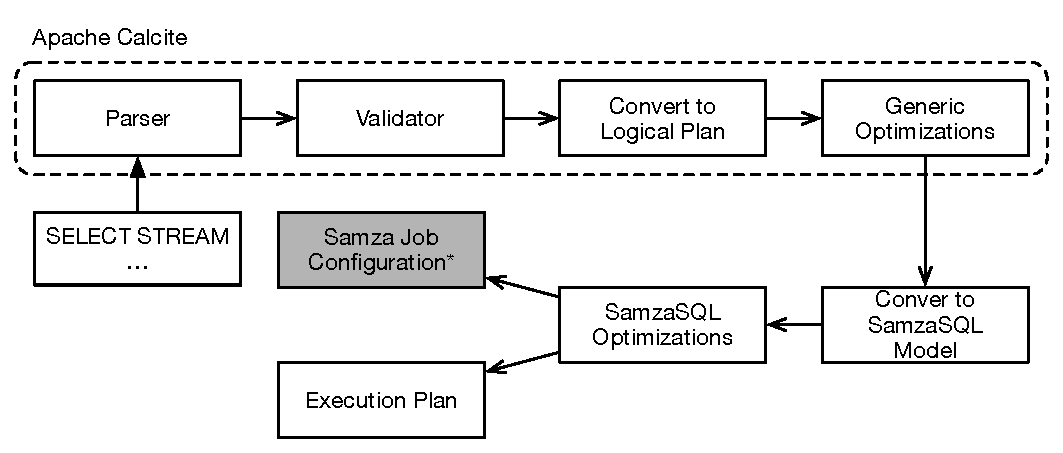
\includegraphics[width=0.9\linewidth]{query-planner.pdf}
	\end{figure}
\end{frame}

\section{Evaluation}

\begin{frame}[c]{Evaluation - Environment}
\begin{itemize}
	\item 100 byte messages (based on previous Kafka benchmarks) 
	\item 3 node (EC2 r3.2xlarge) Kafka cluster
	\item 3 node (EC2 r3.2xlarge) YARN cluster
	\item Each r3.2xlarge instance has 8 vCPUs, 61GB of RAM and 160 GB SSD backed storage
	\item Data model
		\begin{itemize}
			\item Stream - \texttt{Orders (rowtime, productId, orderId, units)} 
			\item Table - \texttt{Products (productId, name, supplierId)} 
		\end{itemize}
\end{itemize}
\end{frame}

%-=-=-=-=-=-=-=-=-=-=-=-=-=-=-=-=-=-=-=-=-=-=-=-=
%	FRAME:
%-=-=-=-=-=-=-=-=-=-=-=-=-=-=-=-=-=-=-=-=-=-=-=-=

\begin{frame}[c]{Evaluation - Filter Throughput}
\begin{figure}
		\centering
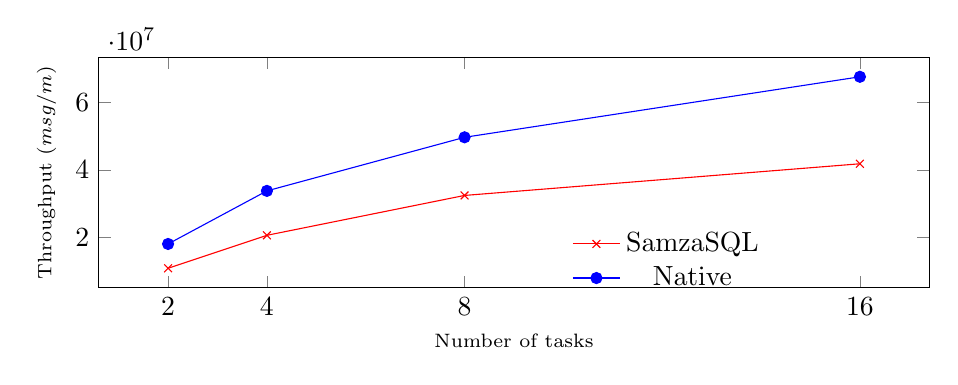
\begin{tikzpicture}
\begin{axis}[
  width=\linewidth,
  height=4.5cm,
  legend style={fill=none,at={(axis cs:10,25000000)},anchor=north west,draw=none},
  ylabel={\scriptsize Throughput ($msg/m$)},
  xlabel={\scriptsize Number of tasks},
    ylabel near ticks,
  xtick={2,  4, 8, 16}]
\addplot[color=red,mark=x] coordinates {
  (2,    5482110.5 * 2)
  (4,   5175536.5 * 4)
  (8, 4059675.125 * 8)
  (16, 2614152.533 * 16)
};

\addplot[color=blue,mark=*] coordinates {
  (2,    9073209.5 * 2)
  (4,   8455300.875 * 4)
  (8, 6205716 * 8)
  (16, 4219658.563 * 16)
};

\legend{SamzaSQL, Native}
\end{axis}
\end{tikzpicture}
\caption{\scriptsize\textbf{\texttt{SELECT STREAM * FROM Orders WHERE units > 50}}}
\end{figure}
\end{frame}

%-=-=-=-=-=-=-=-=-=-=-=-=-=-=-=-=-=-=-=-=-=-=-=-=
%	FRAME:
%-=-=-=-=-=-=-=-=-=-=-=-=-=-=-=-=-=-=-=-=-=-=-=-=

\begin{frame}[c]{Evaluation - Project Throughput}
\begin{figure}
		\centering
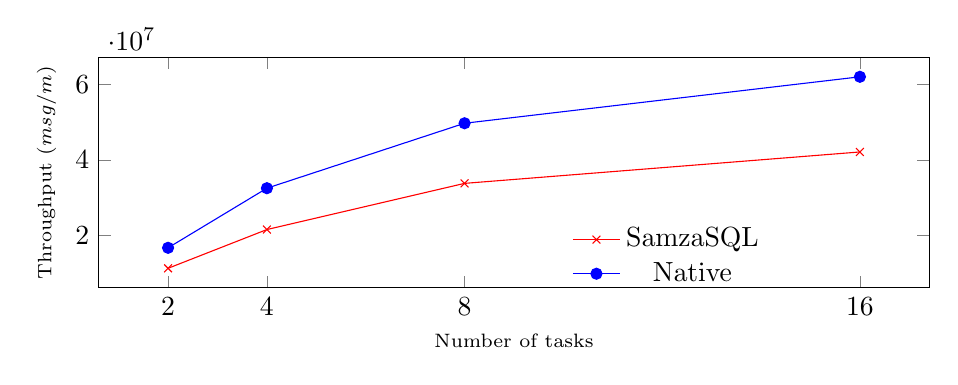
\begin{tikzpicture}
\begin{axis}[
width=\linewidth,
  height=4.5cm,
  legend style={fill=none,at={(axis cs:10,25000000)},anchor=north west,draw=none},
  ylabel={\scriptsize Throughput ($msg/m$)},
  xlabel={\scriptsize Number of tasks},
    ylabel near ticks,
  xtick={2,  4, 8, 16}]
\addplot[color=red,mark=x] coordinates {
  (2,    5630902.5 * 2)
  (4,   5382646.75 * 4)
  (8, 4220770.625 * 8)
  (16, 2630563.5 * 16)
};

\addplot[color=blue,mark=*] coordinates {
  (2,    8344509 * 2)
  (4,   8121428.875 * 4)
  (8, 6211850.5 * 8)
  (16, 3875347.375 * 16)
};

\legend{SamzaSQL, Native}
\end{axis}
\end{tikzpicture}
\caption{\scriptsize\textbf{\texttt{SELECT STREAM rowtime, productId, units FROM Orders}}}
\end{figure}
\end{frame}

%-=-=-=-=-=-=-=-=-=-=-=-=-=-=-=-=-=-=-=-=-=-=-=-=
%	FRAME:
%-=-=-=-=-=-=-=-=-=-=-=-=-=-=-=-=-=-=-=-=-=-=-=-=

\begin{frame}[c]{Evaluation - Stream-to-Relation Join Throughput}
\begin{figure}
		\centering
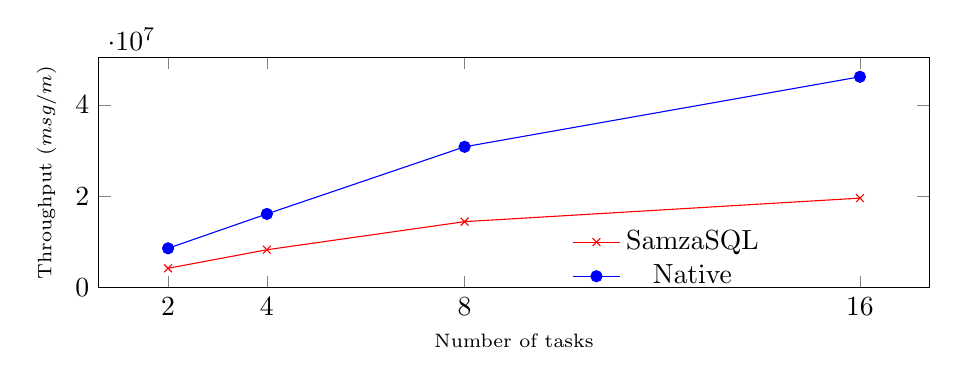
\begin{tikzpicture}
\begin{axis}[
width=\linewidth,
  height=4.5cm,
  legend style={fill=none,at={(axis cs:10,15000000)},anchor=north west,draw=none},
  ylabel={\scriptsize Throughput ($msg/m$)},
  xlabel={\scriptsize Number of tasks},
  ylabel near ticks,
  xtick={2,  4, 8 , 16}]
  
\addplot[color=red,mark=x] coordinates {
  (2,   2095344.333 * 2 )
  (4,   2063065.75 * 4)
  (8, 1800993.5 * 8)
  (16, 1222632.938 * 16)
};

\addplot[color=blue,mark=*] coordinates {
  (2,    4283866.25 * 2)
  (4,   4024959.25 * 4)
  (8, 3850826.733 * 8)
  (16, 2883865.125 * 16)
};
\legend{SamzaSQL,Native}
\end{axis}
\end{tikzpicture}
\caption{\scriptsize\textbf{\texttt{SELECT STREAM Orders.rowtime, Orders.orderId, Orders,productId, Orders.units, Products.supplierId FROM Orders  JOIN ON Orders.productId = Products.productId}}}
\end{figure}
\end{frame}

%-=-=-=-=-=-=-=-=-=-=-=-=-=-=-=-=-=-=-=-=-=-=-=-=
%	FRAME:
%-=-=-=-=-=-=-=-=-=-=-=-=-=-=-=-=-=-=-=-=-=-=-=-=

\begin{frame}[c]{Evaluation - Sliding Window Throughput}
\begin{figure}
		\centering
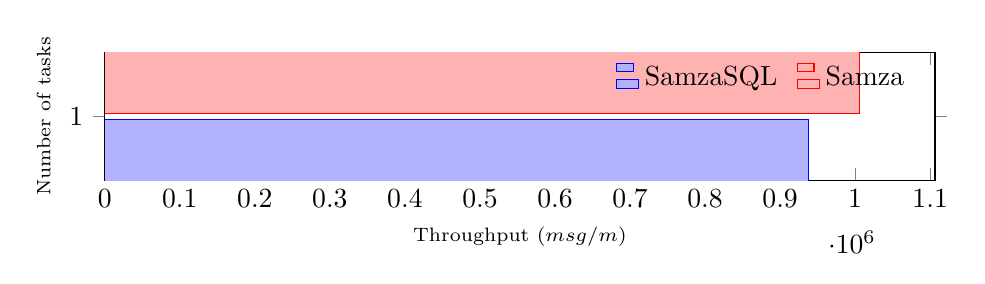
\begin{tikzpicture}
\begin{axis}[xbar,xmin=0,bar width=8,legend columns=2,legend style={
                    % the /tikz/ prefix is necessary here...
                    % otherwise, it might end-up with `/pgfplots/column 2`
                    % which is not what we want. compare pgfmanual.pdf
            /tikz/column 2/.style={
                column sep=5pt,
            },
            draw=none
        },ytick=data,height=3.2cm,legend cell align=left,width=\linewidth,legend style={fill=none},xlabel={\scriptsize Throughput ($msg/m$)},
ylabel={\scriptsize Number of tasks},    ylabel near ticks]
\addplot
coordinates
	{(937608,1)};
\addplot
coordinates
	{(1005827,1)};
  \legend{SamzaSQL, Samza}
\end{axis}
\end{tikzpicture}
\caption{\scriptsize\textbf{\texttt{SELECT STREAM rowtime, productId, units, SUM(units) OVER (PARTITION BY productId ORDER BY rowtime RANGE INTERVAL '5' MINUTE PRECEDING) unitsLastFiveMinutes FROM Orders}}}
\end{figure}
\textcolor{red}{\textit{Sliding window query throughput was measured in a iMac due to limitations in EC2 IO rates.}}
\end{frame}

\begin{frame}[c]{Evaluation}
\begin{itemize}
	\item SamzaSQL underperform 30-40\% compared to native Samza applications mainly due to message format transformations required for streaming SQL runtime
	\item SamzaSQL join underperform mainly due to local store message serialization/deserialization overheads
	\item Local storage effects the throughputs directly

\end{itemize}
\end{frame}


\section{Future Work and Conclusion}


\begin{frame}{Future Work}
\begin{itemize}
	\item Ordering guarantees in the presence of stream repartitioning 
	\item Code generation to bring SamzaSQL generated physical plans closer to Samza Java API based queries  
	\item Stream-to-relation queries
	\item Streaming query optimizations for fast data management systems
\end{itemize}
\end{frame}


\begin{frame}{Conclusion}

\end{frame}

\end{document}